\chapter{Background}\label{chap:Background}

\begin{figure}[t]
    \centering
    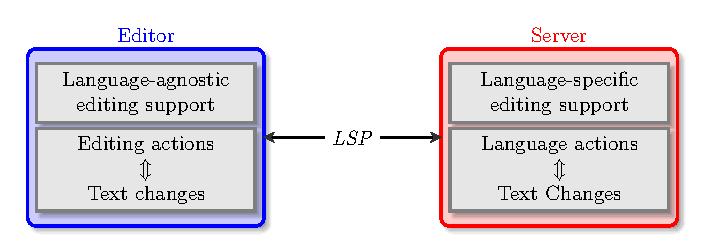
\includegraphics[width=0.9\linewidth]{figs/background/lsp_diagram.pdf}
    \caption{LSP approach to language support. Borrowed from~\cite{Rodriguez-Echeverria18a}}
    \label{lst:lsp}
\end{figure}

In this chapter, we provide an overview of the concepts and technologies that are relevant to the work presented in this thesis. We start by introducing the concept of language servers and the Language Server Protocol (LSP) in Section~\ref{sec:background:LanguageServerProtocol}. We then discuss language workbenches in Section~\ref{sec:bckgnd:language-workbenches}, static analysis and type systems in Section~\ref{sec:background:StaticAnalysisAndTypeSystems}, and software and language product lines in Section~\ref{sec:background:SoftwareAndLanguageProductLines}.

The goal of this chapter is to provide the reader with the necessary background knowledge to understand the work presented in the following chapters. We assume that the reader has a basic understanding of programming languages and software development.

\section{Language Server Protocol}\label{sec:background:LanguageServerProtocol}
The Language Server Protocol\footnote{\url{https://microsoft.github.io/language-server-protocol}} (LSP) is a protocol that allows for the communication between a language server and an editor or an IDE. The LSP is used to decuple the a language-agnostic editor or integrated development environment (IDE) from the language-specific features of a language server (see Listing~\ref{lst:lsp}). This allows for the development of language servers that can be used with multiple editors or IDEs. The LSP is based on the stateless JSON-RPC protocol and defines a set of messages that are used to communicate between the language server and the editor or IDE.

Usually, the LSP Clients are developed as plugins for popular editors or IDEs decresing the effort to support a new language in a given editor. The LSP Clients are responsible for sending requests to the language server and processing the responses. The language server is responsible for providing language-specific features. The LSP defines a set of messages that are used to communicate between the language server and the editor or IDE. These messages include requests for code completion, code navigation, and code analysis, as well as notifications for changes to the document, diagnostics, and progress reports.

Language servers are \textit{de facto} standard for providing language-specific features in editors and IDEs. The LSP is supported by a wide range of editors and IDEs, including Neovim\footnote{\url{https://neovim.io/doc/user/lsp.html}}, Visual Studio Code\footnote{\url{https://code.visualstudio.com/api/language-extensions/language-server-extension-guide}}, Eclipse\footnote{\url{https://www.eclipse.org/community/eclipse_newsletter/2017/may/article1.php}}, and IntelliJ IDEA\footnote{\url{https://plugins.jetbrains.com/docs/intellij/language-server-protocol.html}}. There are several language servers available for popular programming languages, including Rust, TypeScript, Python, and Java and most of them are open-source.\footnote{\url{https://microsoft.github.io/language-server-protocol/implementors/servers}}

The LSP is initiated by Microsoft and is now an open standard that is maintained by the Language Server Protocol Working Group. It was designed for the use with the Visual Studio Code editor, but it has since been adopted by other editors and IDEs. The LSP is under open-source license and is available on GitHub\footnote{\url{https://github.com/microsoft/language-server-protocol}}.

Before the advent of LSP and DAP, developers had to implement language support for each editor separately, having the number of combinations to support $\mathbf{L}$ languages in $\mathbf{L} \times \mathbf{E}$, where $\mathbf{E}$ is the number of editors. Currently, the number of combinations to support $\mathbf{L}$ languages is $\mathbf{L} + \mathbf{E}$~\cite{Rodriguez-Echeverria18a}, as the Microsoft LSP and DAP are editor-agnostic, as shown in Figure~\ref{lst:lsp}.

\subsection{JSON-RPC}\label{subsec:background:JSONRPC}
The LSP uses JSON-RPC to communicate between a language server and an editor. JSON-RPC (v2)\footnote{\url{https://www.jsonrpc.org/specification}} is a stateless, light-weight remote procedure call (RPC) \cite{Birrell84} protocol that uses JSON as the data format.

RPC is a protocol that allows a client to call a procedure on a remote server. The client sends a request to the server, and the server sends a response back to the client. The JSON-RPC protocol defines a set of messages that are used to communicate between the client and the server. These messages include requests, responses, and notifications. The JSON-RPC protocol is designed to be simple and easy to implement, making it well-suited for use in web applications and other distributed systems.

JSON-RPC is a JSON based implementation of the RPC protocol. It defines a set of rules for encoding and decoding JSON data, as well as a set of rules for \textit{Request}, \textit{Notification}, and \textit{Response} messages. The messages are sent over a transport layer, such as HTTP or WebSockets. The JSON-RPC protocol is designed to be simple and easy to implement, making it well-suited for use in web applications and other distributed systems.

All messages refer to a \textit{method} that is a string containing the name of the method to be called. The \textit{params} field is an array or object containing the parameters to be passed to the method. Typically, messages are synchronous, meaning that the client waits for a response from the server before continuing. The \textit{id} field is a unique identifier for the message, which is used to match requests with responses. However, the JSON-RPC protocol also supports asynchronous messages, known as notifications, which do not require a response from the server. This is implemented by setting the \textit{id} field to \textit{null}, in which case the server does not send a response back to the client.

The JSON-RPC specification includes the ability for clients to batch multiple requests or notifications by sending them as a list. The server is expected to respond with a corresponding list of results for each request. Additionally, the server has the flexibility to process these requests concurrently.

\subsection{Command Specifications}\label{subsec:background:CommandSpecifications}
The LSP is defined on top of the JSON-RPC protocol described in section \ref{subsec:background:JSONRPC}. In abstract terms, the LSP defines a set of command that can be sent between a client and a server. In the Language Server Protocol Specification,\footnote{https://microsoft.github.io/language-server-protocol/specifications/lsp/3.17/specification} these commands are divided into four categories: \textit{Language Features}, \textit{Text Document Synchronization}, \textit{Workspace Features}, and \textit{Window Features}.

\subsubsection{Language Features}\label{subsec:background:LanguageFeatures}

In the rest of this work, we will use the term \textit{Language Features} in the context of the Langauge Product Lines (LPLs) to refer to the features that are specific to a language.
The \textit{Language Features} provide the smarts of the language server. Usually, the client sends a request to the server to get information about the document as a tuple of \texttt{TextDocument} and \texttt{Position}. \textit{Code comprehension} and \textit{Coding Features} are the two main categories of commands in this category.

Here a brief description of the most important commands in this category:
\begin{itemize}
    \item \texttt{textDocument/completion}: The completion request is sent from the client to the server to compute completion items at a given cursor position. Completion items are presented in the editor's user interface. If computing full completion items is expensive, servers can additionally provide a handler for the completion item resolve request (\texttt{completionItem/resolve}). This request is sent when a completion item is selected in the user interface.
    \item \texttt{textDocument/hover}: The hover request is sent from the client to the server to request hover information at a given text document position. Hover information typically includes the symbol's signature and documentation.
    \item \texttt{textDocument/definition}: The definition request is sent from the client to the server to resolve the definition location of a symbol at a given text document position.
    \item \texttt{textDocument/references}: The references request is sent from the client to the server to resolve project-wide references for the symbol denoted by the given text document position.
    \item \texttt{textDocument/documentHighlight}: The document highlight request is sent from the client to the server to resolve a document highlights for a given text document position. For programming languages, this usually highlights all references to the symbol denoted by the given text document position.
\end{itemize}

\subsubsection{Text Document Synchronization}\label{subsec:background:TextDocumentSynchronization}
The \textit{Text Document Synchronization} commands are used to notify the server of changes to the document. Client support for \texttt{textDocument/didOpen}, \texttt{textDocument/didChange}, \texttt{textDocument/didClose} is mandatory. This includes the ability to fully and incrementally synchronize changes to the document, such as inserting, deleting, and replacing text.

Here a brief description of the most important commands in this category:
\begin{itemize}
    \item \texttt{textDocument/didOpen}: The document open notification signals that the client is now managing a text document. The server should not read the document using its URI. Open notifications are balanced with close notifications, with only one open notification allowed at a time for a document. The server's ability to fulfill requests is unaffected by a document's open or closed status.
    \item \texttt{textDocument/didChange}: The document change notification is sent from the client to the server to signal changes to a text document. In response, the server should compute a new version of the document's content. The server should not rely on the client to send a specific sequence of change events. The server is free to compute the new version of the document on the fly.
    \item \texttt{textDocument/didClose}: The document close notification is sent from the client to the server when the document is no longer managed by the client. The document's URI is no longer valid and the server should not resolve the document using the URI.
    \item \texttt{textDocument/didSave}: The document save notification is sent from the client to the server when the document is saved. The notification is sent after the document has been saved.
\end{itemize}

\subsubsection{Workspace Features}\label{subsec:background:WorkspaceFeatures}
The \texttt{Workspace Features} category includes commands that allow the client to interact with the workspace. The workspace is the collection of open documents and the client's configuration. The workspace commands are used to manage the workspace, such as symbol search, workspace configuration and client configuration.

Here a brief description of the most important commands in this category:
\begin{itemize}
    \item \texttt{workspace/symbol}: The workspace symbol request is sent from the client to the server to list project-wide symbols matching the query string. The request can be used to populate a list of symbols matching the query string in the user interface.
    \item \texttt{workspace/configuration}: The workspace configuration request is sent from the client to the server to fetch configuration settings from the server. The request can fetch configuration settings from the client's workspace or from the server's configuration.
    \item \texttt{workspace/didChangeConfiguration}: The configuration change notification is sent from the client to the server to signal changes to the client's configuration settings. The server should use the new configuration settings to update its behavior.
    \item \texttt{workspace/didChangeWorkspaceFolders}: The workspace folder change notification is sent from the client to the server to signal changes to the workspace's folders. The server should use the new workspace folders to update its behavior.
\end{itemize}

\subsubsection{Window Features}\label{subsec:background:WindowFeatures}

The \texttt{Window Features} category includes commands that allow the client to interact with the window. The window is the client's user interface, such as the editor, the sidebar, and the status bar. The window commands are used to manage the window, such as showing messages, showing notifications, and showing progress.

Here a brief description of the most important commands in this category:
\begin{itemize}
    \item \texttt{window/showMessage}: The show message notification is sent from the server to the client to show a message to the user. The message can be shown in a variety of ways, such as a dialog box, a status bar, or a notification.
    \item \texttt{window/showMessageRequest}: The show message request is sent from the server to the client to show a message to the user and get a response. The message can be shown in a variety of ways, such as a dialog box, a status bar, or a notification.
    \item \texttt{window/logMessage}: The log message notification is sent from the server to the client to log a message. The message can be logged in a variety of ways, such as a console, a file, or a database.
    \item \texttt{window/showMessageRequest}: The show message request is sent from the server to the client to show a message to the user and get a response. The message can be shown in a variety of ways, such as a dialog box, a status bar, or a notification.
\end{itemize}

\subsection{Key Methods Overview}\label{subsec:bacground:KeyMethodsOverview}

Six \textit{key methods} have been identified by langserver organization\footnote{\url{https://langserver.org}} as the most important methods to be implemented by a language server. These capabilities are:
\begin{enumerate}
    \item \textbf{Diagnostic Analyze} source code --- Parse and Type-check the source code to provide diagnostics.
    \item \textbf{Workspace/Document Symbols} --- List all symbols in the workspace.
    \item \textbf{Jump to Definition} --- Find and jump to the definition of a symbol.
    \item \textbf{Find References} --- List all usages of a symbol.
    \item \textbf{Hover Information} --- Show information about a symbol at the cursor.
    \item \textbf{Code Completion} --- Provide completions for a symbol at the cursor.
\end{enumerate}

\subsubsection{Diagnostic Analysis}\label{subsubsec:background:DiagnosticAnalysis}

The diagnostic analysis is the process of parsing and type-checking the source code to provide diagnostics. The diagnostics are used to identify errors and warnings in the source code, such as syntax errors, type errors, and unused variables. The diagnostics are presented to the user in the editor's user interface, such as a list of errors and warnings in the sidebar.

File update and diagnostic analysis are passive. Thay are sent as notifications in order to avoid blocking communication between the client and the server.

In the figure \ref{fig:diagnostic} we can see an example of diagnostics in Neovim generated by the Rust Language Server. It shows a list of errors and suggestions coused by the concatenation of two \texttt{\&str} variables.

\begin{figure}[t]
    \centering
    \fcolorbox{black}{white}{
        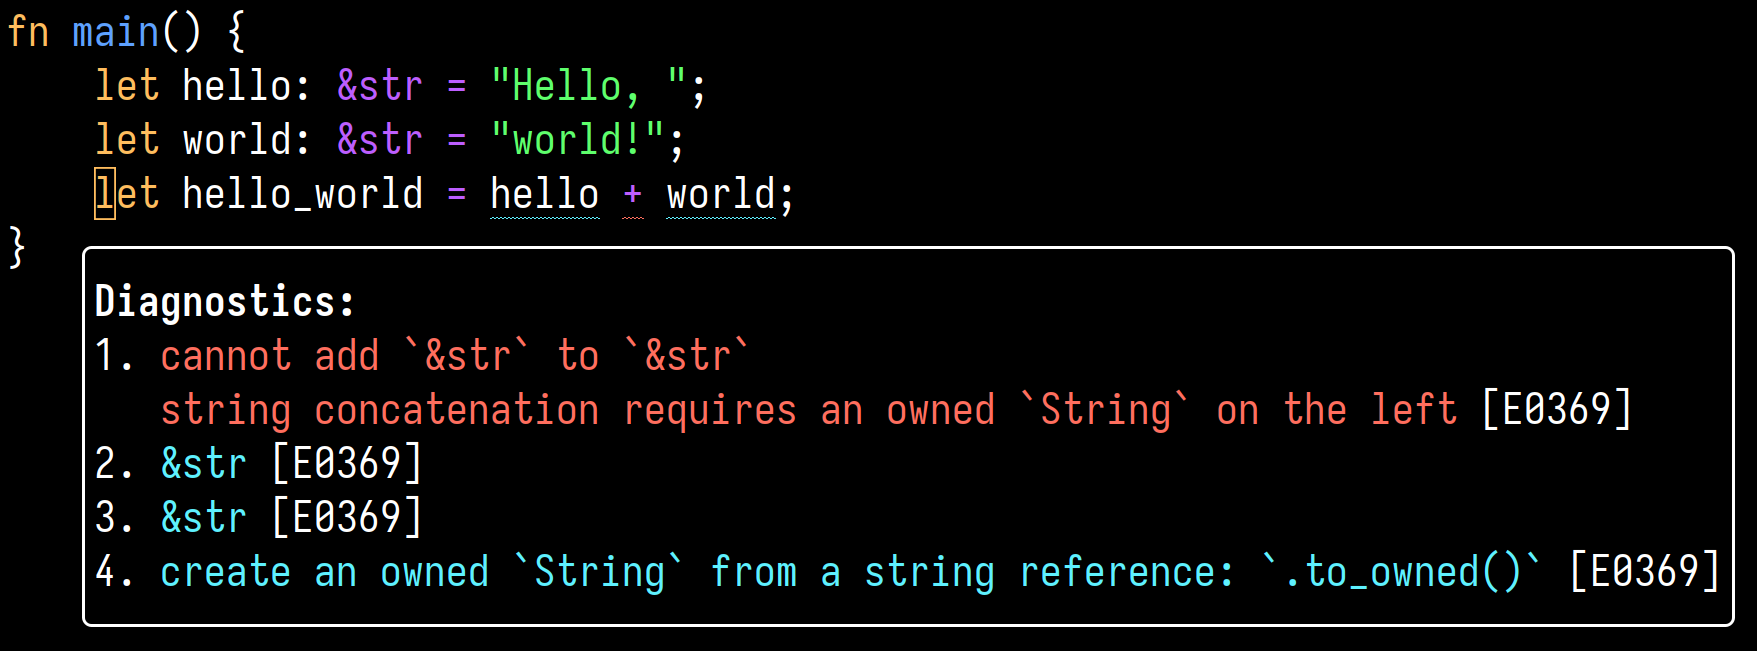
\includegraphics[width=0.9\linewidth]{imgs/background_diagnostic.png}
    }
    \caption{Showing diagnostics in Neovim generated by the Rust Language Server}
    \label{fig:diagnostic}
\end{figure}

\subsubsection{Workspace/Document Symbols}\label{subsubsec:background:WorkspaceDocumentSymbols}

\fbox{
    \parbox{0.95\textwidth}{
        \centering
        \textbf{RPC Method}:  \href{https://microsoft.github.io/language-server-protocol/specifications/lsp/3.17/specification/\#workspace_symbol}{textDocument/workspaceSymbol} or \href{https://microsoft.github.io/language-server-protocol/specifications/lsp/3.17/specification/\#textDocument_documentSymbol}{textDocument/documentSymbol}
    }
}
\hfill \break

\noindent
This feature is defined as both a \textit{Language Feature} and \textit{Workspace Feature}.

The \texttt{textDocument/workspaceSymbol} request is sent from the client to the server to list project-wide symbols matching the query string. The request can be used to populate a list of symbols matching the query string in the user interface. The granularity of the listed symbols depends on the language server implementation.

The difference between \texttt{textDocument/workspaceSymbol} and \texttt{textDocument/documentSymbol} is that the first one takes into account the visibility of the symbols in the workspace showing only the public ones. The second one shows all symbols in the document.


\subsubsection{Jump to Definition}\label{subsubsec:background:JumpToDefinition}
\fbox{
    \parbox{0.95\textwidth}{
        \centering
        \textbf{RPC Method}:  \href{https://microsoft.github.io/language-server-protocol/specifications/lsp/3.17/specification/\#textDocument_definition}{textDocument/definition}
    }
}
\hfill \break

The code navigation is an important feature of the LSP.

The \texttt{textDocument/definition} request is sent from the client to the server to resolve the definition location of a symbol at a given text document position. The server should return the location of the symbol's definition, such as the file path and line number.

In the figure \ref{fig:hover} we can see that at the top of floating window there is the signature of the function \texttt{hello\_world} meaning that the jump to definition will take us to the function definition.

\subsubsection{Find References}
\fbox{
    \parbox{0.95\textwidth}{
        \centering
        \textbf{RPC Method}:  \href{https://microsoft.github.io/language-server-protocol/specifications/lsp/3.17/specification/\#textDocument_references}{textDocument/references}
    }
}
\hfill \break

The retrieval of references is the inverse of the jump to definition explained in the previous section (\ref{subsubsec:background:JumpToDefinition}).

The \texttt{textDocument/references} request is sent from the client to the server to resolve project-wide references for the symbol denoted by the given text document position. The server should return a list of references to the symbol, such as the file path, line number, and the column number.

In Figure \ref{fig:references} we can see that the function \texttt{hello\_world} is being referenced twice in the \texttt{main} function and another occurence is the function definition. In fact, three references are shown in the right window.

\begin{figure}[t]
    \centering
    \fcolorbox{black}{white}{
        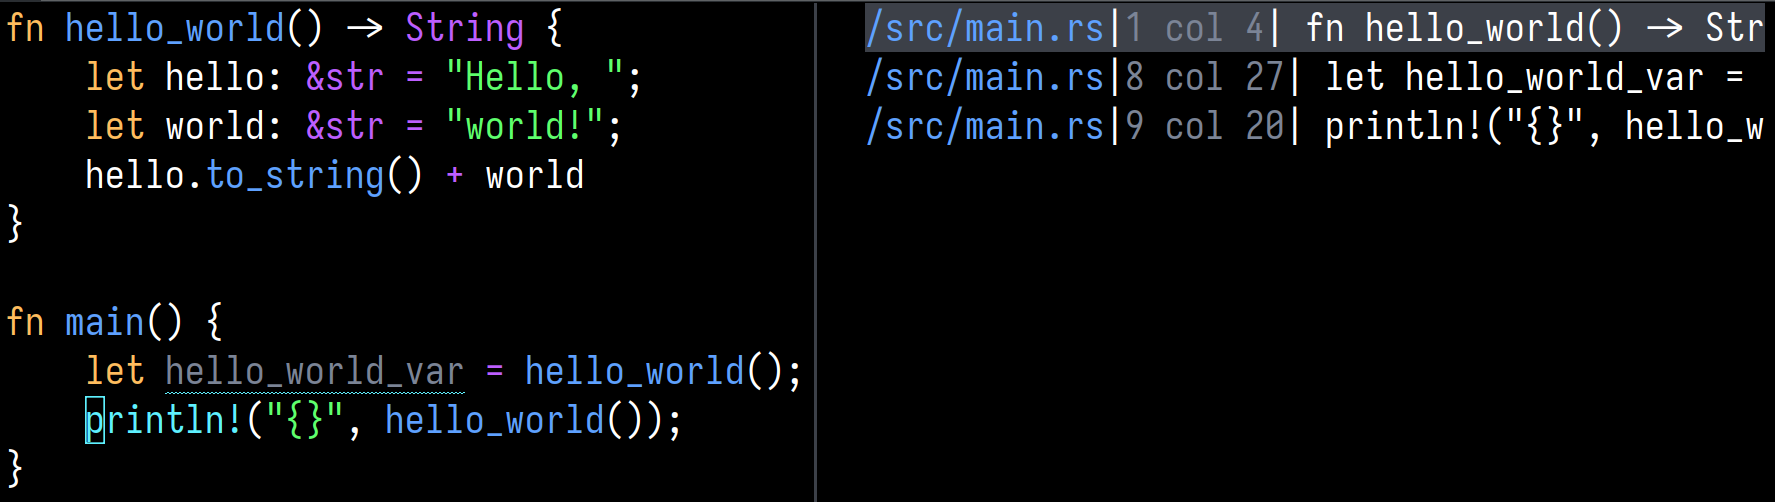
\includegraphics[width=0.9\linewidth]{imgs/background_references.png}
    }
    \caption{Finding references in Neovim generated by the Rust Language Server}
    \label{fig:references}
\end{figure}

\subsubsection{Hover Information}\label{subsubsec:background:HoverInformation}

\fbox{
    \parbox{0.95\textwidth}{
        \centering
        \textbf{RPC Method}:  \href{https://microsoft.github.io/language-server-protocol/specifications/lsp/3.17/specification/\#textDocument_hover}{textDocument/hover}
    }
}
\hfill \break

The hover information is a feature that shows information about a symbol at the cursor. The information typically includes the symbol's signature and documentation. This is triggered by the user hovering the mouse over a symbol in the editor or by pressing a keybinding.

A request is sent from the client to the server to request hover information at a given text document position. The server should return hover information for the symbol at the given position, such as the symbol's signature and documentation.

In the figure \ref{fig:hover} we can see that the function \texttt{hello\_world} is being hovered and the signature of the function is shown in the floating window. The signature is \texttt{fn hello\_world() -> String} and the documentation, written in the comment above the function, is also shown.

\begin{figure}[t]
    \centering
    \fcolorbox{black}{white}{
        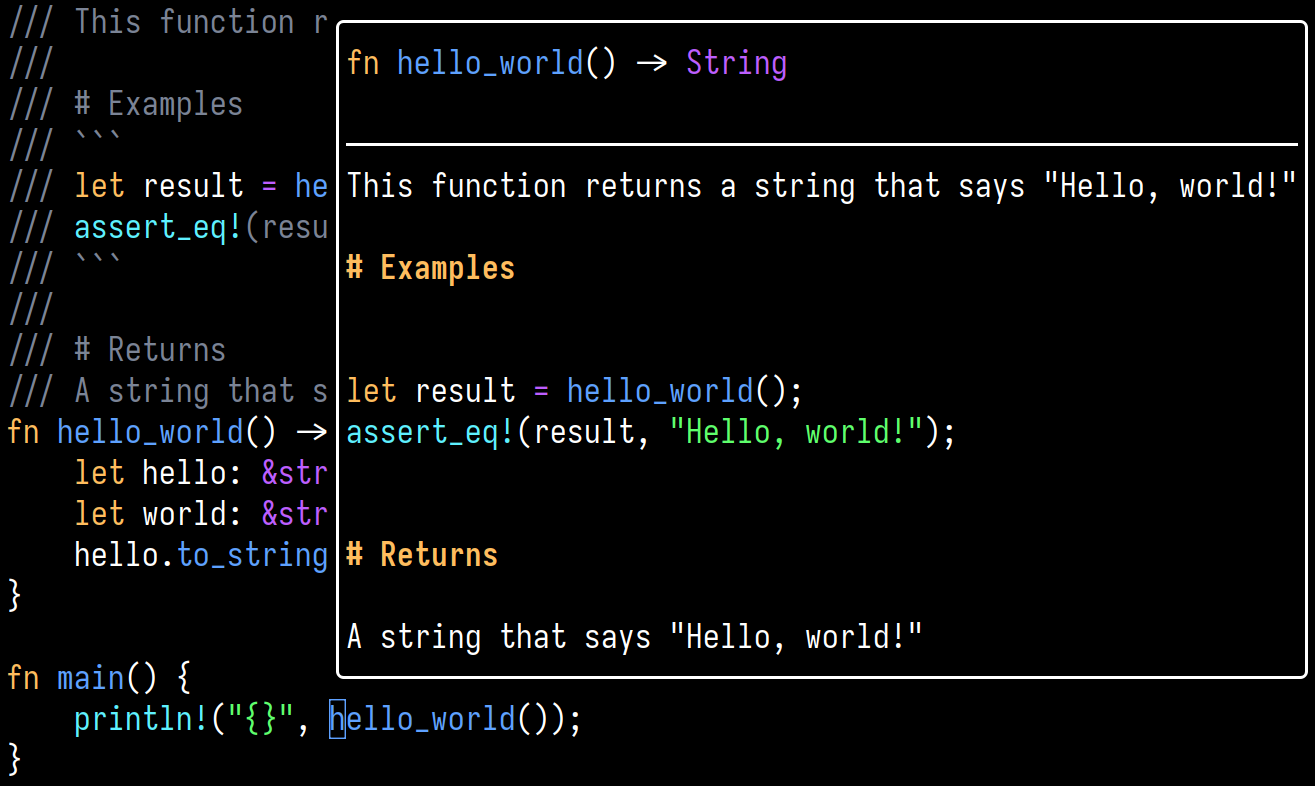
\includegraphics[width=0.9\linewidth]{imgs/background_hover.png}
    }
    \caption{Hover information in Neovim generated by the Rust Language Server}
    \label{fig:hover}
\end{figure}

\subsubsection{Code Completion}\label{subsubsec:background:CodeCompletion}
\fbox{
    \parbox{0.95\textwidth}{
        \centering
        \textbf{RPC Method}:  \href{https://microsoft.github.io/language-server-protocol/specifications/lsp/3.17/specification/\#textDocument_completion}{textDocument/completion}
    }
}
\hfill \break

The code completion is a feature that provides completions for a symbol at the cursor. The completions are presented in the editor's user interface. If computing full completion items is expensive, servers can additionally provide a handler for the completion item resolve request (\texttt{completionItem/resolve}). This request is sent when a completion item is selected in the user interface.

Usually, the completion is triggered by the user typing a character or pressing a keybinding in proximity to a character, such as \texttt{.}, \texttt{::}, or \texttt{->}.

In the figure \ref{fig:completion} we can see that the code completion is triggered by the user typing \texttt{to\_} and pressing \texttt{<C-n>} in the editor. Two float windows are shown with the completion items. The first one shows the options for the \texttt{to\_} function associated with the \texttt{\&str} type and the second one shows the documentation of the selected completion item.

\begin{figure}[h]
    \centering
    \fcolorbox{black}{white}{
        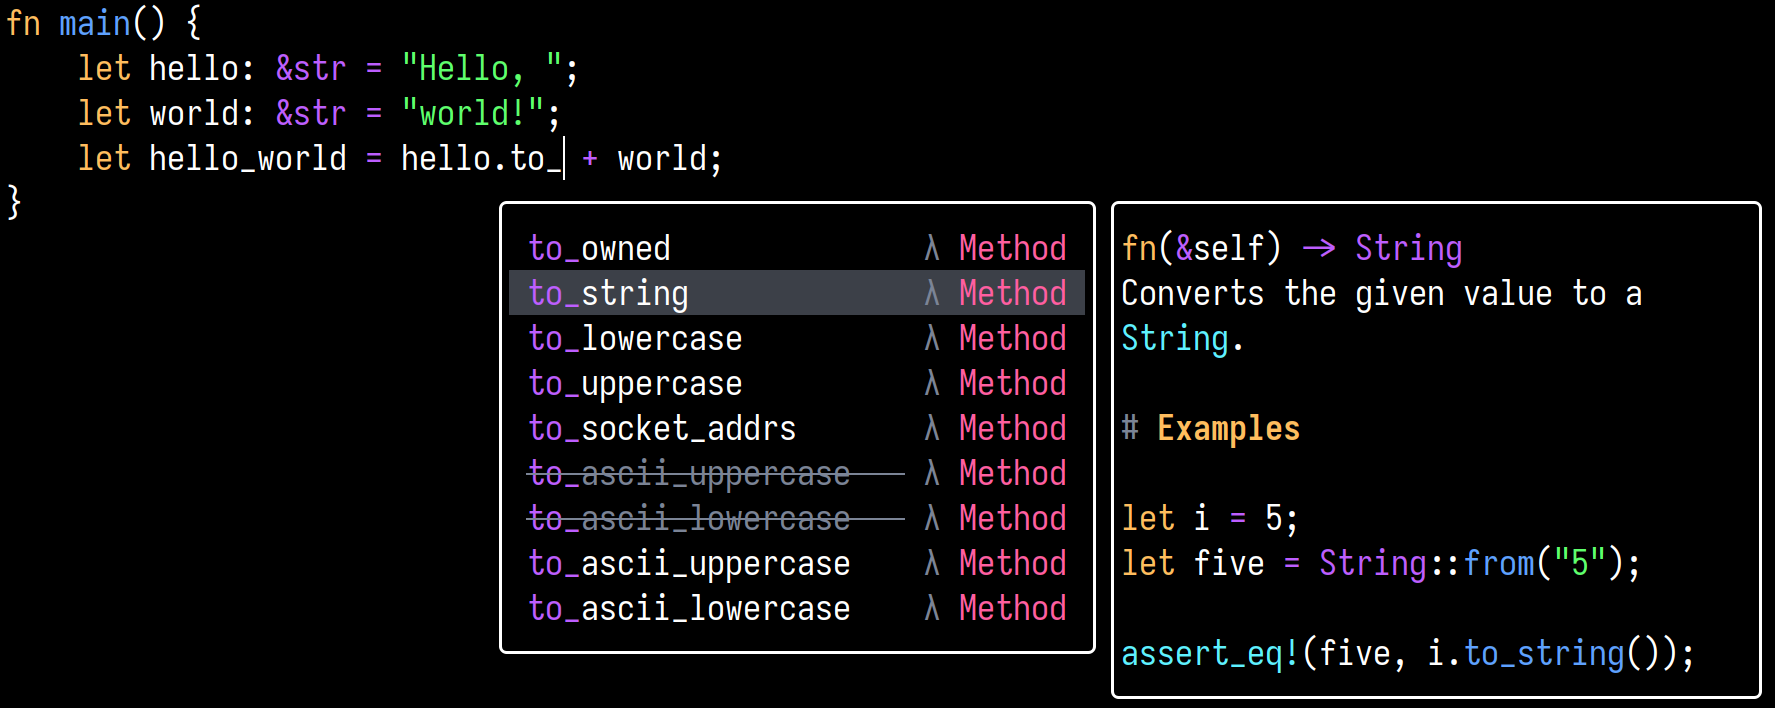
\includegraphics[width=0.9\linewidth]{imgs/background_completion.png}
    }
    \caption{Code completion in Neovim generated by the Rust Language Server}
    \label{fig:completion}
\end{figure}

\subsection{Approaches to Source Code Analysis}\label{subsec:background:ApproachesToSourceCodeAnalysis}
Language servers handle source code analysis using various methods, influenced significantly by the complexity of the language. The choice of approach affects how servers process file indexes, manage changes, and respond to requests.

The Language Server Protocol (LSP) supports two methods for sending updates: diffs of atomic changes and complete transmission of changed files. The former requires incremental parsing and analysis, which are challenging to implement but enable much faster processing of files upon changes. Incremental parsing relies on an internal representation of the source code that allows efficient updates for small changes. This method necessitates providing the parser with the right context to correctly parse a changed fragment of code.

In practice, most language servers re-index the entire file when changes occur, discarding the previous internal state. This approach is more straightforward to implement as it poses fewer requirements for the architects of the language server, but it is significantly less performant. Unlike incremental processing, which updates only the affected portions of its internal structure, even minor changes such as adding or removing lines require reprocessing the entire file. This method may suffice for small languages and codebases but becomes a performance bottleneck with larger ones.

For code analysis, LSP implementers must choose between lazy and greedy approaches to processing files and answering requests. Greedy implementations resolve most available information during the file's initial indexing, enabling the server to answer requests using simple lookups. Conversely, lazy approaches resolve only minimal local information during indexing, invoking ad-hoc resolution for requests and possibly memoizing the results for future use. Lazy resolution is more common with incremental indexing, as it reduces the work associated with file changes, which is crucial for complex languages that would otherwise require a significant amount of redundant work.

\section{Language Workbenches}\label{sec:bckgnd:language-workbenches}

The term \textit{Language Workbench} was coined by Martin Fowler in 2005~\cite{Fowler05} to describe a set of tools that support the development of domain-specific languages (DSLs) in the context of \textit{language-oriented programming} paradigm~\cite{Ward94}.

A language workbench will typically include tools to support the definition, reuse and composition of domain-specific languages together with their integrated development environment (IDE).

Current language workbenches usually support:
\begin{itemize}
    \item Specification of the language concepts or metamodel
    \item Specification of the editing environments for the domain-specific language
    \item Specification of the execution semantics, e.g. through interpretation and code generation
\end{itemize}

Language workbenches have been developed for various technological spaces, but they all share the same focus developing programming languages and having a strong emphasis on code resuability and separation of concerns.

 Some of the most popular language workbenches are:
\begin{itemize}
    \item \textbf{JetBrains MPS}\footnote{\url{https://www.jetbrains.com/mps/}}: A powerful language workbench that allows the creation of domain-specific languages and the generation of code from them.~\cite{Campagne14, Voelter12}
    \item \textbf{Xtext}\footnote{\url{https://www.eclipse.org/Xtext/}}: A framework for developing domain-specific languages and languages for code generation.~\cite{Zhang23}
    \item \textbf{Spoofax}\footnote{\url{https://www.metaborg.org/en/latest/}}: A language workbench for developing textual domain-specific languages.~\cite{Visser10, Kats10b, Wachsmuth14}
    \item \textbf{MontiCore}\footnote{\url{https://www.monticore.de/}}: A language workbench for developing domain-specific languages and language families.~\cite{Krahn08, Gronninger08, Krahn10, Rumpe21}
\end{itemize}

\texttt{Neverlang} (Sect.~\ref{subsec:background:neverlang}) will be discussed with particular detail, since most of the research discussed in this dissertation will use \texttt{Neverlang} as a running example.

\subsection{Neverlang}\label{subsec:background:neverlang}

\begin{Listing}[t]
	\setminted[neverlang]{escapeinside=@@}
	\showneverlang*{Backup.nl}\vskip -10pt%
	\caption{Syntax and semantics for the backup task. Borrowed from \cite{Cazzola20}}
    \label{lst:backup}
	\newcommand{\nt}[1]{%
		\node[draw, fill=none, shape=circle, inner sep=0pt, minimum width=.375cm] (c\i) at (s\i) {};%
		\coordinate (d\i0p) at ($(d\i0)+(-1pt,2pt)$);% chktex 1
		\coordinate (d\i1p) at ($(d\i1)+(1pt,-3pt)$);% chktex 1
		\node[draw, thick, shape=rectangle, name=d\i, inner sep=1pt, fit=(d\i0p) (d\i1p)] {};% chktex 1 % chktex 36
	}
	\begin{tikzpicture}[overlay, thick, BloodRed]
		\coordinate (s0) at ($(s0)+(2pt,0pt)$) ;
		\foreach \i in {0, 1, 2} {%
			\nt{\i}
			\draw[-stealth, rounded corners=7pt] (c\i) -- (d\i);
		}
	\end{tikzpicture}
\end{Listing}

The \textit{Neverlang} \cite{Cazzola12c, Cazzola13e, Cazzola15c} framework promotes the code reusability and the separation of concerns in the implementation of programming languages, based upon the concept of \textit{language-feature}.
The basic development unit is the \textbf{module}, as shown in line 1 of Listing \ref{lst:backup}.
A module may contain a \textbf{reference syntax} and could have zero or more \textbf{role}s. A role, used to define the semantics, is the unit of composition that defines actions that should be executed when some syntax is recognized, as defined by \textit{syntax-directed translation} \cite{Aho86}.
Syntax definitions are defined using \textit{Backus–Naur form} (BNF) grammars, represented as sets of \textit{productions} and \textit{terminals}.
Syntax definitions and semantic \textbf{role}s are tied together using \textit{slice}s.
Listing \ref{lst:backup} shows a simple example of a Neverlang module implementing a backup task of the \texttt{LogLang} LPL. Reference syntax is defined in lines 2-6; the \textit{categories} (line 5) are used also to generate the syntax highlighting for the IDEs.
Semantic actions may be attached to a non-terminal using the production's name as a reference, or using the position of the non-terminal in the grammar, as shown in line 8, numbering start with 0 from the top left to the bottom right.
The two \textit{String} non-terminals on the right-hand side of the \textit{Backup} production are referenced using 1 and 2, respectively.
Different semantic actions may be attached to the same production thanks to the multiplicity of \textbf{role}s that can be defined for a module. Each \textbf{role} is a compilation phase that can be executed in a specific order, as shown in line 24.
In contrast, the \texttt{BackupSlice} (lines 14-18) reveals how the syntax and semantics are tied together; choosing the \texttt{concrete syntax} from the Backup module (line 15), and two \texttt{role}s from two different modules (lines 16-17).
Finally, the \texttt{language} can be created by composing multiple \textbf{slices} (line 20).
The composition in Neverlang is twofold \cite{Cazzola20}: between modules and between slices. Thus, the grammars are merged in order to generate the complete language parser. On the other hand, the semantic actions are composed in a pipeline, and each \textbf{role} traverses the syntax tree in the order specified in the \textbf{roles} clause (line 24).
Please see \cite{Cazzola15c} for a more detailed explanation of the \texttt{Neverlang} framework.


\section{Static Analysis and Type Systems}\label{sec:background:StaticAnalysisAndTypeSystems}

Static code analysis is a software verification technique that refers to the process of examining the code without executing it in order to capture the defects in the code early avoiding costly later fixations \cite{Aurum02}. Static code analysis has two main approaches: manual and automated \cite{Ilyas16}.
Manual code analysis is a time-consuming process that requires human expertise to review the code and identify defects. Automated code analysis, on the other hand, uses tools to analyze the code and identify defects automatically. Automated code analysis tools can be used to analyze the code for defects such as syntax errors, type errors, and logic errors. These tools can also be used to enforce coding standards and best practices, such as naming conventions, code formatting, and code complexity.

\subsection{Type Systems}\label{subsec:background:TypeSystems}

\textit{Type systems} are a fundamental part of static code analysis. A type system~\cite{Pierce02} is a set of rules that defines how types are used in a programming language. The type system defines the types of variables, functions, and expressions, as well as the rules for type compatibility and type inference.

\textit{Type checking} is the process of verifying that the types of variables, functions, and expressions are used correctly in the code. Type checking can be done \textit{statically}, at compile time, or \textit{dynamically}, at runtime. Static type checking is more efficient and catches type errors earlier in the development process, while dynamic type checking is more flexible and allows for more dynamic programming.

\textit{Type inference} is the process of automatically deducing the types of variables, functions, and expressions in the code. Type inference is used to reduce the amount of type annotations required in the code, making the code more concise and easier to read. Type inference is used in statically typed languages such as OCaml, Java, and Rust, as well as in dynamically typed languages such as Python and JavaScript, see table~\ref{tab:TypeSystems}.

\begin{table}[t]
    \rowcolors{2}{gray!25}{white}
    % \setlength\arrayrulewidth{0pt}
    \centering
    \begin{tabular}{ c c c c }
        \\\toprule \textbf{Language} & \textbf{Type System} & \textbf{Type Checking} & \textbf{Type Inference} \\
        \midrule
        C & Weak & Static & No \\
        OCaml & Strong & Static & Yes \\
        Java & Strong & Static  & Yes \\
        Rust & Strong & Static  & Yes \\
        Python & Strong & Dynamic  & Yes \\
        JavaScript & Weak & Dynamic  & Yes \\
        Haskell & Strong & Static  & Yes \\
        Erlang & Strong & Dynamic  & Yes \\
        Perl & Weak & Dynamic  & No \\
        \bottomrule
    \end{tabular}
    \caption{Examples of programming languages and their type systems}
    \label{tab:TypeSystems}
\end{table}

A programming language can be classified based on its type system and type checking. There are two main categories of type systems: \textit{strong} and \textit{weak}. A strong type system enforces type safety and does not allow for implicit type conversions, while a weak type system allows for implicit type conversions and does not enforce type safety. A programming language can also be classified based on its type checking: \textit{static} or \textit{dynamic}. Static type checking is done at compile time and catches type errors before the code is executed, while dynamic type checking is done at runtime and catches type errors as the code is executed.

In table \ref{tab:TypeSystems} we show examples of programming languages and their type systems. C is a statically typed language with a weak type system, meaning that it allows for implicit type conversions and does not enforce type safety. OCaml, Java, and Rust are statically typed languages with strong type systems, meaning that they enforce type safety and do not allow for implicit type conversions. Python and JavaScript are dynamically typed languages with strong type systems, meaning that they enforce type safety at runtime. Haskell is a statically typed language with a strong type system and support for type inference. Erlang is a dynamically typed language with a strong type system and support for type inference.

\subsection{Theoretical Aspects}\label{subsec:background:TheoreticalAspects}

Theoretical aspects of type systems are an important research area in computer science. Type systems are used to ensure the correctness and safety of programs by enforcing rules about how types are used in the code. Type systems can be classified based on their properties, such as \textit{soundness}, \textit{completeness}, and \textit{decidability}.

A brief explanation of these properties is given below:
\begin{itemize}
    \item A type system is \textbf{sound} if it guarantees that well-typed programs do not produce errors. Soundness is an important property of a type system because it ensures that the type system is correct and that it enforces the correct use of types in the code.
    \item A type system is \textbf{complete} if it can infer the type of any expression in the code. Completeness is an important property of a type system because it ensures that the type system can handle all possible expressions in the code.
    \item A type system is \textbf{decidable} if it can determine the type of any expression in a finite amount of time. Decidability is an important property of a type system because it ensures that the type system is efficient and can be used in practice.
\end{itemize}

\subsection{Type Theory as a Logic}\label{subsec:background:TypeTheoryAsALogic}

A \textit{Type theory} is a mathematical logic, which is to say it is a collection of rules of inference that result in judgments.
Most logics are based on judgements, which are statements that assert the truth of a proposition.
Martin-L\"of in \textit{Intuitionistic Type Theory}~\cite{Martin84} introduced a new type theory, previously published in 1972, that is based on the idea of judgments as the central concept of the theory.
In Martin-L\"of's~\cite{Martin96} type system, a judgment is no longer just an affirmation or denial of a proposition, but a general act of knowledge. When reasoning mathematically we make judgments about mathematical objects. One form of judgment is to state that some mathematical statement is true. Another form of judgment is to state that something is a mathematical object, for example a set~\cite{sep-type-theory-intuitionistic}.

In the following sections, we will discuss the basic concepts of type theory and how it is used in the context of programming languages.

\subsubsection{Judgements}\label{subsubsec:background:Judgements}

Martin-L\"of type theory has four basic forms of judgment and is a considerably more complicated system than first-order logic.

The four basic forms of judgments are:
\begin{itemize}
    \item $\vdash A \textrm{ type}$ --- This judgment asserts that $A$ is a well-formed type.
    \item $\vdash a : A$ --- This judgment asserts that $a$ is an element of type $A$.
    \item $\vdash A = B \textrm{ type}$ --- This judgment asserts that $A$ and $B$ are equal types.
    \item $\vdash a = b : A$ --- This judgment asserts that $a$ and $b$ are equal elements of type $A$.
\end{itemize}

In programming languages, the first two judgments are used to define the types of variables and functions, while the last two judgments are used to define equality between types and elements.
Below, an example showing the usage of each of the four basic forms of judegment.
$$
\vdash \texttt{Int} \textrm{ type} \quad \vdash 1 : \texttt{Int} \quad \vdash \texttt{Int} = \texttt{Int} \textrm{ type} \quad \vdash 1 = 1 : \texttt{Int}
$$

\subsubsection{Contexts}\label{subsubsec:background:Contexts}

In general, judgments are \textit{hypothetical}, meaning that they are made under certain assumptions. These assumptions are kept track of in a \textit{context}.
In Martin-L\"of's type theory, the context is a list $x_1 : A_1, \ldots, x_n : A_n$ of variables and their types. Note that the context is ordered, meaning that the order of the variables matters.

The four basic forms of judgments are made in the context of a given context $\Gamma$:
\begin{itemize}
    \item $\Gamma \vdash A \textrm{ type}$ --- This judgment asserts that $A$ is a well-formed type in the context $\Gamma$.
    \item $\Gamma \vdash a : A$ --- This judgment asserts that $a$ is an element of type $A$ in the context $\Gamma$.
    \item $\Gamma \vdash A = B \textrm{ type}$ --- This judgment asserts that $A$ and $B$ are equal types in the context $\Gamma$.
    \item $\Gamma \vdash a = b : A$ --- This judgment asserts that $a$ and $b$ are equal elements of type $A$ in the context $\Gamma$.
\end{itemize}

In programming languages, the context is used to keep track of the types of variables and functions in the code. For instance,
$$
x : \texttt{Int}, y : \texttt{Int} \vdash x + y : \texttt{Int}
$$
or,
$$
x : \texttt{Int}, y : \texttt{Int} \vdash x + y = y + x : \texttt{Int}
$$

\subsubsection{Inference Rules}\label{subsubsec:background:InferenceRules}
Let $\Pi$ be a set of type functions in the form of $\Pi x : A. B$ where $x$ is a variable of type $A$ and $B$ is a type.

The first type of inference rule in Martin-L\"of's type theory is the \textit{formation rule}.
\begin{tcolorbox}[myboxstyle=black, title=Formation Rule]
     This rules define how types are formed and how elements are formed in a given context. The formation rule is used to define the types of variables and functions in the code.
    \begin{prooftree}
        \AxiomC{$\Gamma \vdash A \textrm{ type}$}
        \AxiomC{$\Gamma, x : A \vdash B \textrm{ type}$}
        \BinaryInfC{$\Gamma \vdash \Pi x : A. B \textrm{ type}$}
    \end{prooftree}
    \tcblower
    Written in natural language, the $\Pi$-formation rule states that if $A$ is a type in the context $\Gamma$ and $B$ is a type in the context $\Gamma, x : A$, then $\Pi x : A. B$ is a type in the context $\Gamma$.
\end{tcolorbox}

The second type of inference rule in Martin-L\"of's type theory is the \textit{introduction rule}.
\begin{tcolorbox}[myboxstyle=black, title=Introduction Rule]
    This rule define how elements are introduced in a given context. The introduction rule is used to define the elements of variables and functions in the code.
    \begin{prooftree}
        \AxiomC{$\Gamma, x : A \vdash b : B$}
        \UnaryInfC{$\Gamma \vdash \lambda x : A. b : \Pi x : A. B$}
    \end{prooftree}
    \tcblower
    Written in natural language, the $\Pi$-introduction rule states that if $b$ is an element of type $B$ in the context $\Gamma, x : A$, then $\lambda x : A. b$ is an element of type $\Pi x : A. B$ in the context $\Gamma$.
\end{tcolorbox}


The third type of inference rule in Martin-L\"of's type theory are the \textit{elimination rule}.
\begin{tcolorbox}[myboxstyle=black, title=Elimination Rule]
    This rule define how elements are eliminated in a given context. The elimination rule is used to define the elimination of variables and functions in the code.
    \begin{prooftree}
        \AxiomC{$\Gamma \vdash f : \Pi x : A. B$}
        \AxiomC{$\Gamma \vdash a : A$}
        \BinaryInfC{$\Gamma \vdash f a : B[x := a]$}
    \end{prooftree}
    \tcblower
    Written in natural language, the $\Pi$-elimination rule states that if $f$ is an element of type $\Pi x : A. B$ in the context $\Gamma$ and $a$ is an element of type $A$ in the context $\Gamma$, then $f a$ is an element of type $B[x := a]$ in the context $\Gamma$.
\end{tcolorbox}

The fourth type of inference rule in Martin-L\"of's type theory are the \textit{equality rule}.
\begin{tcolorbox}[myboxstyle=black, title=Equality Rule]
    This rule define how types and elements are equal in a given context. The equality rules are used to define the equality of types and elements in the code.

    In the following $B[x := a]$ denotes the substitution of $a$ for $x$ in $B$.
    \begin{prooftree}
        \AxiomC{$\Gamma, x : A \vdash b : B$}
        \AxiomC{$\Gamma \vdash a : A$}
        \BinaryInfC{$\Gamma \vdash (\lambda x : A. b) a = b[x := a] : B[x := a]$}
    \end{prooftree}
    \tcblower
    Written in natural language, the $\Pi$-equality rule states that if $b$ is an element of type $B$ in the context $\Gamma, x : A$ and $a$ is an element of type $A$ in the context $\Gamma$, then $(\lambda x : A. b) a$ is equal to $b[x := a]$ in the context $\Gamma$.
\end{tcolorbox}

\subsection{Type Inference in Programming Languages}\label{subsubsec:background:TypeInferenceInProgrammingLanguages}

Given the typing environment $\Gamma$, the type inference algorithm uses the rules of type theory to deduce the types of variables, functions, and expressions in the code. The type inference algorithm is used to determine the types of variables and functions in the code, as well as to check the correctness of the code.

\begin{Listing}[t]
    \centering
    \mbox{
        \showrust*[.45\textwidth]{typeinference.rs}
        \quad
        \showml*[.45\textwidth]{typeinference.ml}
    }
    \caption{Example of type inference in Rust and OCaml}
    \label{lst:background:typeinference}
\end{Listing}

In listing~\ref{lst:background:typeinference} we show an example of type inference in Rust and OCaml. In both examples, the type inference algorithm is used to deduce the types of the variables \texttt{z} in the code. In case of Rust code (line 5), the type of \texttt{z} is inferred to be \texttt{i32} because the types of \texttt{x} and \texttt{y} are known to be \texttt{i32}. In case of OCaml code (line 3), the type of \texttt{z} is inferred to be \texttt{int} because the types of \texttt{x} and \texttt{y} are known to be \texttt{int}.


\section{Domain-Specific Languages}\label{sec:background:DomainSpecificLanguages}

According to~\cite{Mernik05}, many software language are \textit{domain specific} rather than general purpose. They can be classified in:
\begin{itemize}
    \item application oriented~\cite{Sammet69},
    \item special purpose~\cite{Ross78},
    \item specialized~\cite{Bergin96},
    \item task specific~\cite{Nardi93}, and
    \item application languages~\cite{Martin85},
\end{itemize}
Application language are called also \textit{fourth-generation languages}~\cite{Martin85}, and an example is SQL~\cite{Codd70} used to query databases.

Domain specific languages (DSLs) are languages that are designed to be used in a specific domain or application area. DSLs are used to express concepts and operations that are specific to a particular domain. DSLs are typically more expressive and easier to use than general-purpose programming languages, making them well-suited for developing software with respect to the problems of a particular application domain~\cite{VanDeursen00}.

According to~\cite{Favalli23}, the usage of DSLs brings several benefits, such as:
\begin{itemize}
    \item \textit{encapsulation} -- DSLs allow developers to encapsulate domain-specific knowledge in the language, making it easier to understand and use.
    \item \textit{productivity} -- DSLs can improve productivity by providing higher-level abstractions that are closer to the problem domain.
    \item \textit{communication} -- DSLs can improve communication between domain experts and developers by providing a common language for discussing requirements and specifications.
    \item \textit{quality} -- DSLs provide a way to express domain-specific constraints and requirements, which can help improve the quality of the software.
\end{itemize}

\subsection{Internal and External DSLs}\label{subsec:background:InternalAndExternalDSLs}

\begin{Listing}[t]
    \centering
    \showscala*[\textwidth]{calc_internal.scala}
    \caption{An internal DSL for arithmetic expressions in Scala}
    \label{lst:background:addexpr-internal}
\end{Listing}

DSLs are classified as internal (or embedded~\cite{Fowler10}) and external. Internal DSLs are an idiomatic way of writing code in a general purpose programming language. They are not require a special parser or compiler, but they are limited by the syntax and semantics of the host language.
Some programming languages, such as Lisp~\cite{Fowler05}, Ruby~\cite{Fowler10} and Scala~\cite{Artho15}, intrinsically support the development of internal DSLs.
External DSLs, on the other hand, are standalone languages that require a separate parser and compiler. They are more flexible and expressive than internal DSLs, but they are also more complex to develop and maintain.

In figure~\ref{lst:background:addexpr-internal} we show an example of an internal DSL for arithmetic expressions in Scala. The DSL uses the Scala syntax to define arithmetic expressions, such as addition, subtraction, multiplication, and division. The DSL is embedded in the Scala programming language, allowing developers to write code that looks like a domain-specific language but is actually valid Scala code.
It can be seen that no special parser or compiler is required to use the DSL, as it is written in Scala and can be executed using the Scala interpreter.
Line 10 in ~\ref{lst:background:addexpr-internal} shows an example of using the DSL to define an arithmetic expression; the expression is syntact sugar for the Scala code \inlinescala{calc.add(5).multiply(3).subtract(1).divide(2)}.

\begin{Listing}[t]
    \centering
    \showscala*[0.9\textwidth]{calc_external.scala}
    \caption{An external DSL for arithmetic expressions in Scala}
    \label{lst:background:addexpr-external}
\end{Listing}

In contrast, in figure~\ref{lst:background:addexpr-external} we show an example of an external DSL for arithmetic expressions in Scala. The DSL implementation is more complex than the internal DSL, as it requires a separate parser and compiler to process the DSL code. The DSL uses a custom syntax to define arithmetic expressions, such as \texttt{add}, \texttt{subtract}, \texttt{multiply}, and \texttt{divide}. The DSL is defined using a parser combinator library in Scala, which allows developers to define the syntax and semantics of the DSL in a declarative way.

\section{Software and Language Product Lines}\label{sec:background:SoftwareAndLanguageProductLines}

Variability in products is common in industrial production. For instance, in a car factory, a base car model can be customized with various options such as different colors, a navigation system, a cooling system, and parking sensors. This type of industrial production, known as variability-rich production, has been managed in traditional engineering environments through the development of product lines.

\textit{Software Product Line Engineering} (SPLE)~\cite{Van01, Van07} is a software engineering methodology that extends the concept of product lines to software development, following the dream of massive software reuse. The objective of SPLE is to find similarities among software products and to manage the variability in the software development process.

At the same time, a \textit{software family} can be obtained using SPL~\cite{Clements01} by defining a set of features. A feature can be a \textit{core} feature, which is mandatory for all products in the family, or an \textit{variable} feature, which can be included or excluded from the product. The set of features defines the \textit{feature model} of the software family.

\subsection{Feature Variability}\label{subsec:background:FeatureVariabilityInSPL}

Feature variability is a key concept in SPL. They are often developed using a \textit{feature-oriented programming}~\cite{Prehofer97} (FOP) paradigm, which allows developers to define features as first-class entities in the code. In this context, each feature represents either functional or non-functional characteristics of a subset of the software family's members. However, there is no universally accepted formal definition of software features. Typically, a feature is informally described as an increment~\cite{Batory21}. Therefore, an SPL can be viewed as a collection of all available features, while a product configuration is a valid subset of the SPL. Each configuration corresponds to a specific member of the software family. Although various approaches to expressing SPLs exist in the literature, \textbf{feature models}~\cite{Kang90} (FMs) are considered the \textit{de facto} standard for variability modeling~\cite{Czarnecki12}.
An FM is a tree-like structure that represents the features of a software family and their relationships. The root of the tree represents the software family, and the node represents a feature. The edges represent the relationships between the features.
It is important to note that, given a FM, a software variant is identified through a configuration, which is a set of features that are selected from the FM. A configuration is valid if it satisfies all the constraints defined in the FM.

\begin{figure}[t]
    \centering
    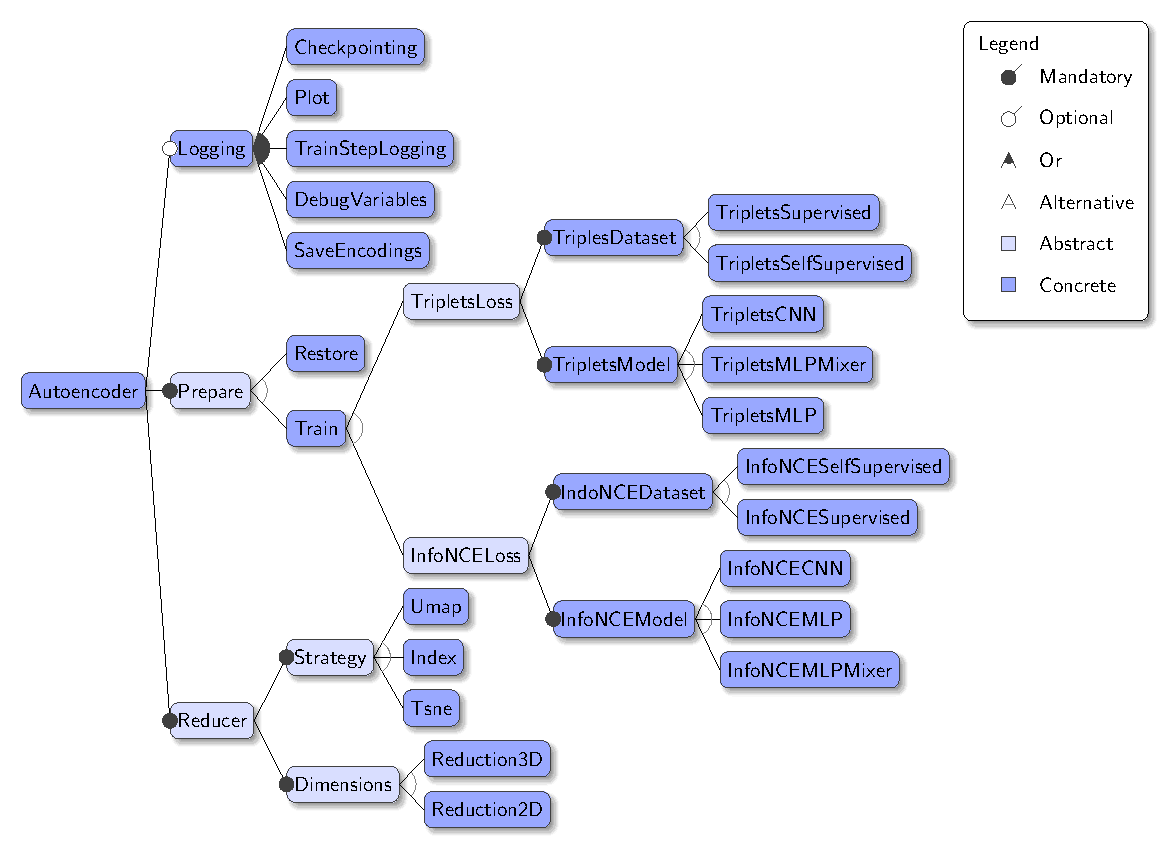
\includegraphics[width=0.9\linewidth]{figs/background/mnist_featuremodel.pdf}
    \caption{FM of a family of neural networks used to encode the MNIST dataset, taken from \cite{Cazzola22c}}
    \label{lst:background:featuremodel}
\end{figure}

Figure~\ref{lst:background:featuremodel} shows an example of an FM for a family of neural networks used to encode the MNIST dataset.
FM structures implicitly define dependencies among features. Features can be \textit{abstract} (\texttt{Reducer} and \texttt{Prepare} in Fig~\ref{lst:background:featuremodel}) or \textit{concrete} (\texttt{Logging} and \texttt{Train} in Fig~\ref{lst:background:featuremodel}).
An abstract feature represents a group of related features, while a concrete feature represents a specific functionality.
Features are \textit{mandatory} -- such as \texttt{Dimension} in Fig~\ref{lst:background:featuremodel} -- if they must be included if their parent feature is selected, \textit{optional} if they can be included or excluded.
Features that are part of a group can be put in an \textit{alternative} or \textit{or} relationship.Or-relationship (children of Logging node in Fig.~\ref{lst:background:featuremodel}) means that only one of the features in the group can be selected, while an alternative relationship (children of Train node in Fig.~\ref{lst:background:featuremodel}) means that at least one of the features in the group must be selected if the parent feature is selected.

Dependencies can be explicitly defined using cross-tree constraints -- i.e., Boolean expression among features of the FM~\cite{Cazzola22c}, where each features represents a term in the expression. Each term is true if the corresponding feature is active in the current configuration and false otherwise. Cross-tree constraints support general Boolean operators such as AND, OR, NOT, IMPLIES, and IFF with their traditional meanings.
The expressiveness of these constraints allows for defining dependencies that span the entire feature model, rather than being limited to parent-child relationships. A configuration is considered invalid if any cross-tree constraint evaluates to false or if the transposition of the tree into a prepositional formula is not satisfiable, including the father-son relationships and the mandatory features.

An example of a cross-tree constraint is the following, where $\Rightarrow$ represents the implication operator:
\begin{equation*}
    \texttt{Train} \Rightarrow \texttt{Logging} \vee \texttt{Strategy}
\end{equation*}

Implicit and explicit dependencies among features can lead to issues such as dead features (features that can never be activated), false-optional features (features labeled as optional but are actually required), and atomic sets (groups of features that must either all be activated or all be deactivated in any given configuration). Conducting static analysis of Feature Models (FMs) to identify these anomalies can enhance the quality of Software Product Lines. This research area encompasses both structural~\cite{TerBeek21} and behavioral~\cite{Benavides10} methodologies.
 Additionally to FOP, other paradigms for SPLE such as aspect-oriented programming (AOP)~\cite{Groher09} and delta-oriented programming (DOP)~\cite{Koscielny14} exist.

\subsection{Language Product Lines}\label{subsec:background:LanguageProductLines}

\textit{Language Product Lines} (LPLs)~\cite{Mendez-Acuna16, Cazzola16i, Cazzola15f, Cazzola13g} are a specialization of SPLs that focus on the variability of programming languages. Researchers and practitioners have gained interest in LPLs~\cite{Cazzola17, Ghosh11b, Kuehn14} due to the increasing complexity of software systems and the need for more efficient and effective ways to manage variability in programming languages.
LPLs are used to manage the variability in the syntax and semantics of programming languages. In particular, a family of programming languages can be defined using an LPL, where each language in the family is a member of the software family. The variability in the family is managed using features, which represent the different syntax and semantics of the languages in the family.

\begin{Listing}[t]
    \centering
    \showneverlang*[0.9\textwidth]{AddExpr.nl}
    \caption{Example of a Neverlang module for the addition expression}
    \label{lst:background:addexpr}
\end{Listing}

LPLs enable developers to efficiently generate and maintain multiple language variants within a coherent framework.
In this context, any language workbenches, such as Neverlang, adopt the LPL approach to manage the variability~\cite{Klint09b, Cazzola13g} and the modularization of the syntax and semantics of programming languages.

Since LPLs are an engineering methodology for creating languages, researchers have also concentrated on assessing the quality of these LPLs. This assessment involves proposing various software metrics~\cite{Cazzola21b}. Additionally, there is an emphasis on mutation operators for mutation testing of LPLs, as outlined in~\cite{Cazzola22b}.

Listing~\ref{lst:background:addexpr} shows an example of a Neverlang module for the addition expression. The module defines the syntax and semantics of the addition expression in the \texttt{ExprLang} language. The module contains a reference syntax, which defines the syntax of the addition expression, and a role, which defines the semantics of the addition expression.
In the reference syntax bock, using the \textbf{provides} keyword, the module defines the features exported by the module. The keyword \textbf{requires}, instead, is used to import features from other modules, defining indirectly the dependencies among modules.

\begin{figure}[t]
    \centering
    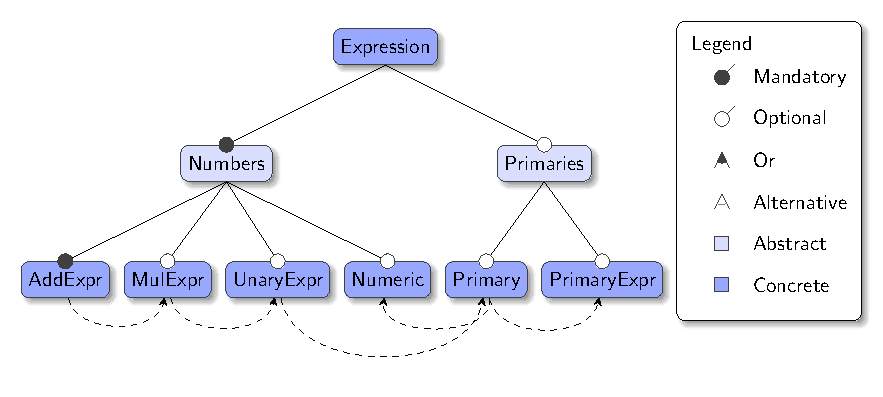
\includegraphics[width=0.9\linewidth]{figs/background/expression_featuremodel.pdf}
    \caption{Feature Model for the expression language, taken from \cite{Cazzola15f}}
    \label{lst:background:exprfeaturemodel}
\end{figure}

In Figure~\ref{lst:background:exprfeaturemodel}, we show an example of an FM for a family of expression languages. In the figure the \textit{cross-tree constraints} are shown as dashed lines connecting the features. The cross-tree constraints are used to define dependencies among features that are not explicitly defined in the FM. For instance, the cross-tree constraint between the \texttt{AddExpr} and \texttt{MulExpr} features states that if the \texttt{AddExpr} feature is selected, then the \texttt{MulExpr} feature must also be selected, for more details see~\cite{Cazzola15f}.
Anyway, using the code in Listing~\ref{lst:background:addexpr} it it trivial to see the cross-tree constraints from \texttt{AddExpr} node to \texttt{MulExpr}, because of the \texttt{requires} keyword in the reference syntax block.


